%%%%%%%%%%%%%%%%%%%%%%%%%%%%%%%%%%%%%%%%%%%%%%%%%%%%%%%%%%%%%%%%%%%%%%%%%%%%%%%%%%%%%%%%%%%%%%%%%%%%%%%%%%%%%%%%%%%%%%%%%%%%%%%%%%%%%%%%%%%%%%%%%%%%%%%%%%%%%%%%%%%%%%%%%%%%%%%%%%%%%%%%%%%%
% Written By Michael Brodskiy
% Class: AP Statistics
% Professor: M. Thompson
%%%%%%%%%%%%%%%%%%%%%%%%%%%%%%%%%%%%%%%%%%%%%%%%%%%%%%%%%%%%%%%%%%%%%%%%%%%%%%%%%%%%%%%%%%%%%%%%%%%%%%%%%%%%%%%%%%%%%%%%%%%%%%%%%%%%%%%%%%%%%%%%%%%%%%%%%%%%%%%%%%%%%%%%%%%%%%%%%%%%%%%%%%%%

\documentclass[12pt]{article} 
\usepackage{alphalph}
\usepackage[utf8]{inputenc}
\usepackage[russian,english]{babel}
\usepackage{titling}
\usepackage{amsmath}
\usepackage{graphicx}
\usepackage{enumitem}
\usepackage{amssymb}
\usepackage[super]{nth}
\usepackage{expl3}
\usepackage[version=4]{mhchem}
\usepackage{hpstatement}
\usepackage{rsphrase}
\usepackage{everysel}
\usepackage{ragged2e}
\usepackage{geometry}
\usepackage{fancyhdr}
\usepackage{cancel}
\usepackage{siunitx}
\geometry{top=1.0in,bottom=1.0in,left=1.0in,right=1.0in}
\newcommand{\subtitle}[1]{%
  \posttitle{%
    \par\end{center}
    \begin{center}\large#1\end{center}
    \vskip0.5em}%

}
\DeclareSIUnit\Molar{\textsc{m}}
\usepackage{hyperref}
\hypersetup{
colorlinks=true,
linkcolor=blue,
filecolor=magenta,      
urlcolor=blue,
citecolor=blue,
}

\urlstyle{same}


\title{1.1 Categorical Data}
\date{August 13, 2021}
\author{Michael Brodskiy\\ \small Instructor: Mr. Thompson}

% Mathematical Operations:

% Sum: $$\sum_{n=a}^{b} f(x) $$
% Integral: $$\int_{lower}^{upper} f(x) dx$$
% Limit: $$\lim_{x\to\infty} f(x)$$

\begin{document}

\maketitle

\begin{enumerate}

  \item 

    \begin{enumerate}

      \item The individuals are students (both male and female)

      \item The variables are gender, grade level, GPA, children in family, homework last night (in minutes), and phone preference. The categorical variables are gender, grade level, and phone preference. The quantitative variables are GPA, children in family, and homework last night

    \end{enumerate}

    \setcounter{enumi}{2}

  \item \begin{tabular}{| l | l |} \hline Categorical & Quantitative\\ \hline Movie & Time\\ \hline Year & Box Office\\ \hline Rating  & \\ \hline Genre & \\ \hline   \end{tabular}

    \setcounter{enumi}{4}

  \item \begin{tabular}{| l | l |} \hline Categorical & Quantitative\\ \hline Type of Wood & Paint Thickness\\ \hline Type of Water Repellent & Weathering Time\\ \hline Paint Color & \\ \hline \end{tabular}

    \setcounter{enumi}{6}

  \item \begin{tabular}{| l | l |} \hline Continuous & Discrete\\ \hline Time to complete survey  & Distance from Home\\ \hline & Number of Siblings\\ \hline & Books read in a month \\ \hline \end{tabular}

  \item \begin{tabular}{| l | l |} \hline Continuous & Discrete\\ \hline Time on site & Times site was visited  \\ \hline Time since creation of profile & Likes Received  \\\hline \end{tabular}

    \setcounter{enumi}{10}

    \newpage

  \item

    \begin{enumerate}

      \item The individuals are babies born on a certain day

        \begin{center}

          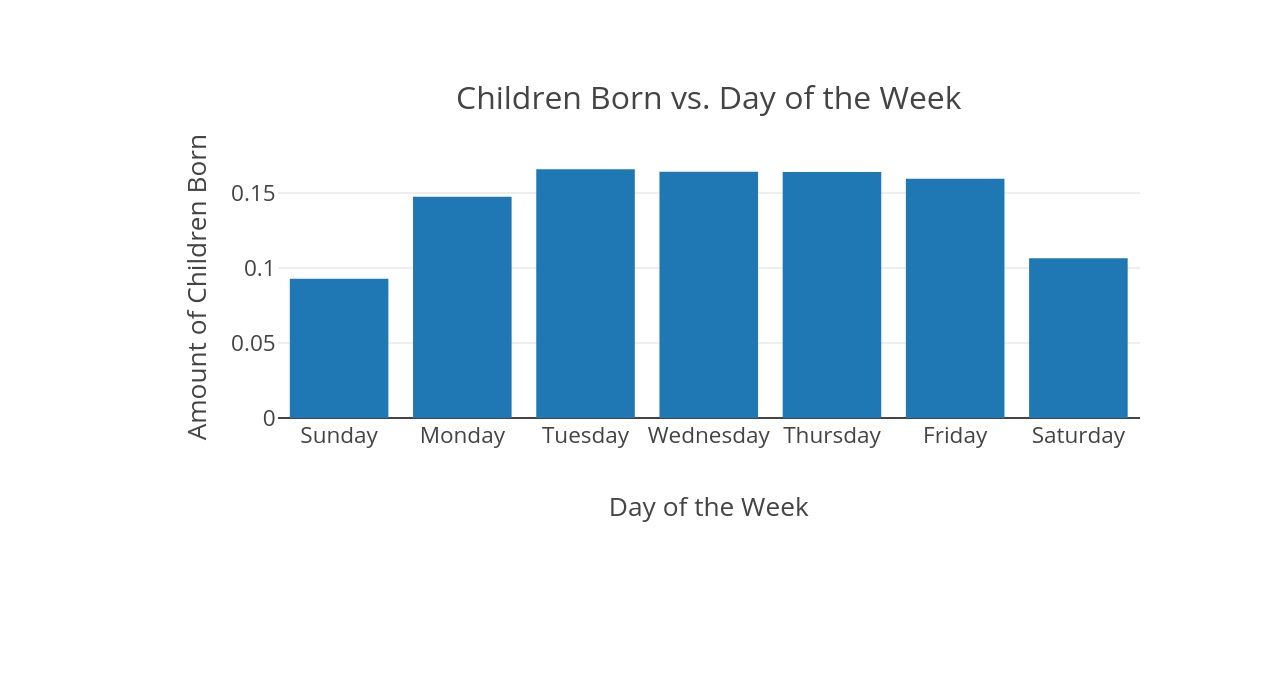
\includegraphics{Figures/1-1-1.png}
          
        \end{center}

      \item According to the graph, the frequency born Tuesday-Friday is approximately equal, and greater than Sunday, Monday, and Saturday

    \end{enumerate}

    \setcounter{enumi}{12}

    \begin{center}

      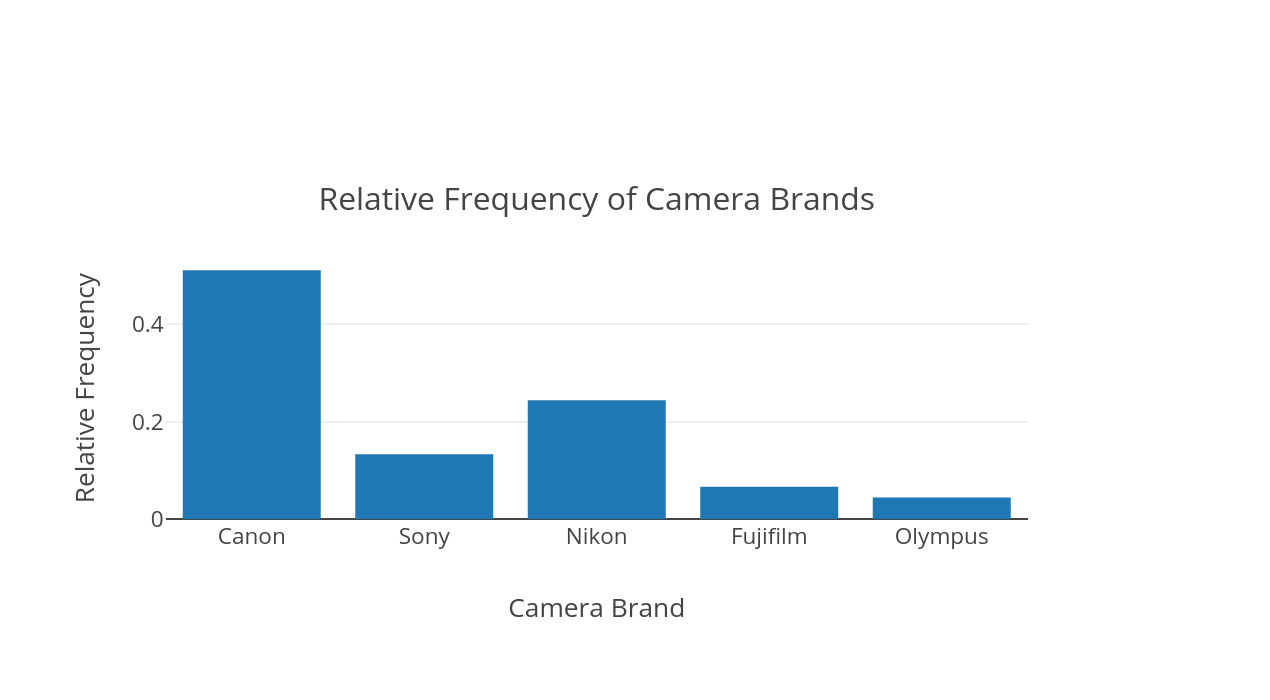
\includegraphics{Figures/1-1-2.png}
      
    \end{center}

  \item Evidently, Canon was purchased at a significantly higher frequency, with Nikon in second, and all other brands much farther behind

\end{enumerate}

\end{document}

